\section{Program Breakdown}

\subsection{Introduction}
The program is written in java, providing a GUI interface to rapidly enable a wide variety of testing conditions. 

\subsection{MainThread}

The MainThread class is what really makes this application tick. As the name
suggest the class provides a thread on which the simulation is ran on. Prior to providing and running a thread, upon initialization, this class does a number of useful things. The first and foremost functionality it carries out is creating all
the Sensors. The number of sensors, as well as the number of sectors, and range is determined by parameters from the GUI, modified by the sliders. Creating Sensor
can be further broken down into three steps; deciding their placement, identifying the Neighbours, and assign the Sensor to and algorithm. <Something about
placement. Either a short description or something saying it's in another
section>.  Two Sensors are identified as Neighbours if both are in range of each other, falling on some sector of each other. Neighbours are identified in the
"record\_neighbours" method in the MainThread. This method is ran at most 
O(n$^{2}$)
times. Each call to this method passes in the index of a Sensor which needs to 
have it's Neighbours identified. The method then loops through all the Sensors up 
until the index passed in, so all the Sensors previously initialized. At each 
iteration of this loop, it checks if the Sensor at the current iteration of the 
loop is in range of the Sensor at the passed in index. If they are in range of 
each other, they are made Neighbours and a prime number is determined from the 168 
possible prime numbers for the Sensor at the passed in index, such that no 
neighbourly Sensors have the same prime number, thus effectively coloring the 
graph of Sensors both graph theory-wise and literally the Sensor's beam color. 
After the Neighbours are determined, each Sensor is assigned to an algorithm, this 
taking O(n) time, as it goes through each Sensor and assigns it to an algorithm. 
The type of algorithm that all the Sensors will be assigned to is determined by a 
parameter from the GUI. After the initialization the MainThread is prepared to 
run.  The run method of the MainThread, runs until the application is stopped and 
does one of the two things and is responsible for spawning the Java thread. It 
either re-initializes the Sensors if the user has pressed New. The main 
functionality that the run method provides is calling on update. In update the 
algorithms are updated, taking an O(n), where n is the amount of algorithms that 
have not yet been complete. An algorithm is complete when there are no remaining 
Neighbours for it's Sensor that need to be connected. Once the algorithm is 
complete it is then moved to another list, that acts an inactive list, so that it 
is on longer updated. This is to done to significantly improve the overall 
performance of the application, since the purpose of the simulation is to 
demonstrate how Sensors discover each other, once a Sensor has discovered all of 
it's neighbourly Sensors there is no need for it to keep searching/being updated. 
After the update has happened on the Algorithms, the Neighbours are checked for 
connection, followed by output to both the GUI and log, and a call to re-draw the 
sensors on the GUI. 

\begin{figure}
\caption{UML Diagram}
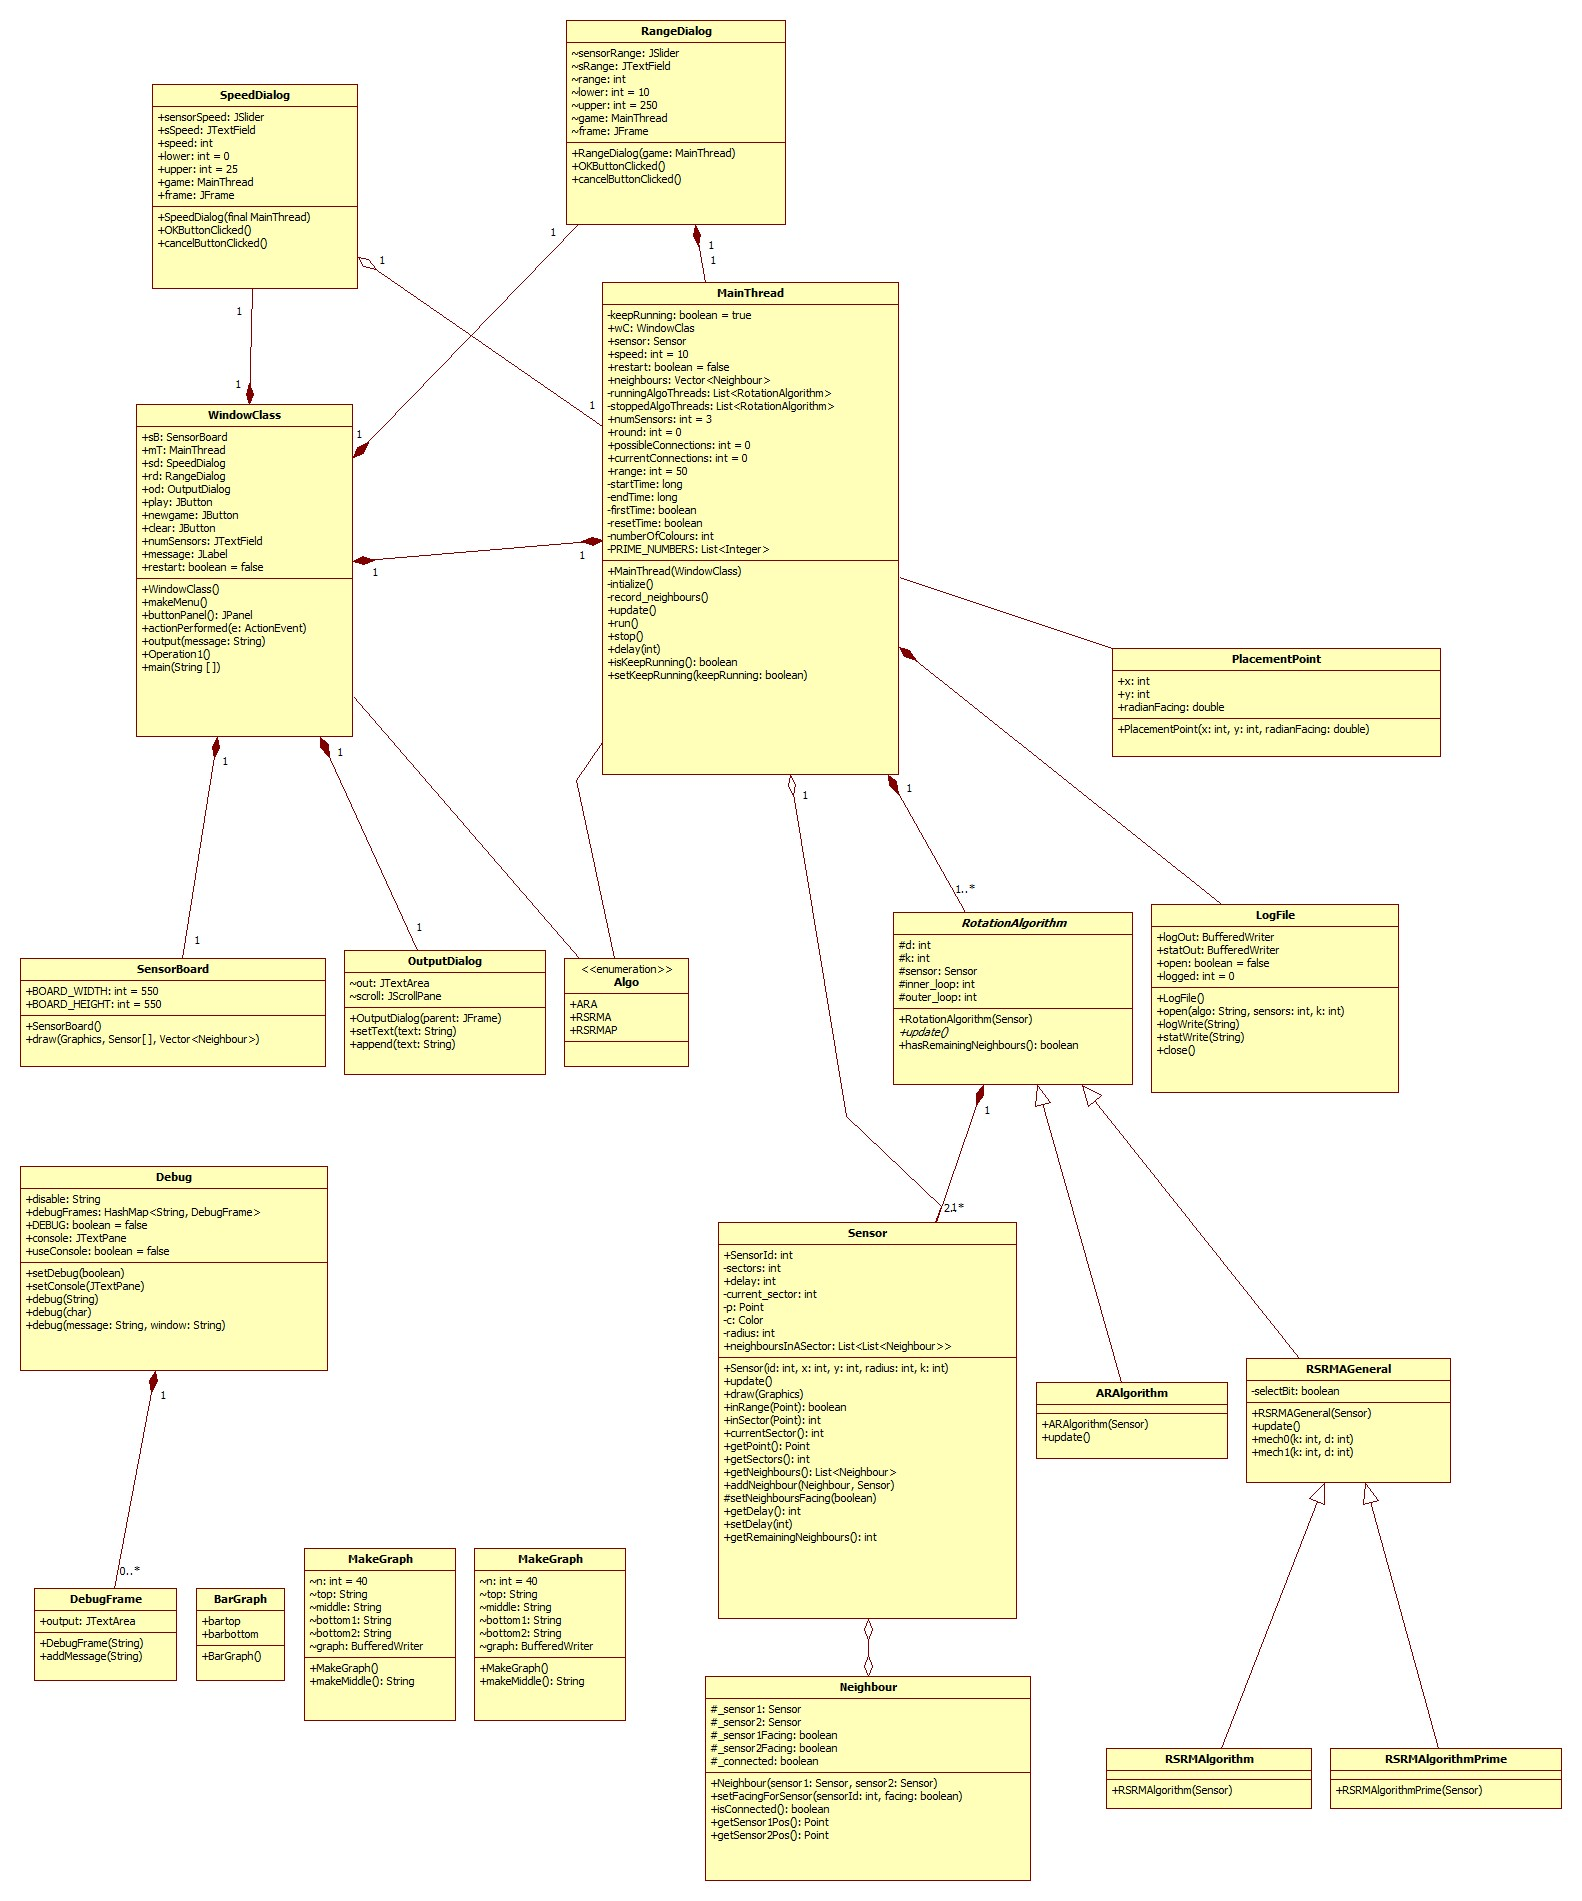
\includegraphics[height = 16cm]{pics/Main.jpg}\\[0.5cm]    
\end{figure}

The current approach MainThread takes for "running" the sensors, is that there is a list of algorithms that are each responsible for "running" their Sensors. The algorithms themselves are all updating in the update method of the MainThread, and the MainThread is the only class responsible for spawning one thread that the repeatedly calls on update. The other approach would have been to allow each individual algorithm to spawn their own threads, which would then "run"/update the Sensors, while the MainThread handles checking Neighbour connects and calling on the GUI re-draw. During the development of this application, we have implemented this method. We've found that allowing each algorithm to have it's own separate thread would cause synchronization problems, would model a more practical simulation. However having just one thread in the MainThread and updating the algorithms in the update method that is repeatedly called on, the way that the runs application now, would model a more theoretical simulation, and thus this way was chosen to better demonstrate how the algorithms function and how the Sensors discover each other.

\subsection{The Interface}

\subsection{Known Issues}
 